\section{扩散指数模型}
\begin{frame}{因子分析是分析高维宏观经济数据的常用手段}

\begin{figure}[H]
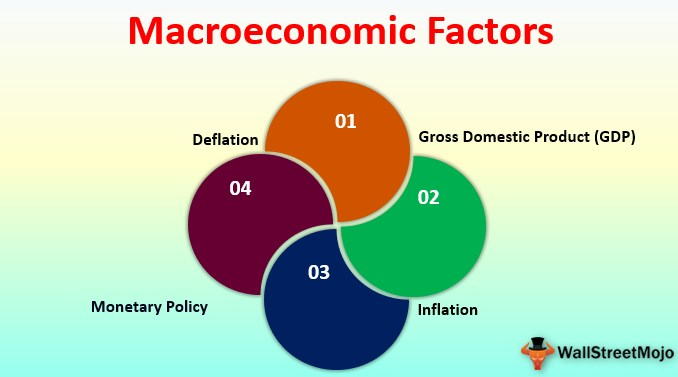
\includegraphics[width=8cm]{pics/macroeco-demo.jpeg}
\end{figure}

\end{frame}

\begin{frame}{扩散指数模型进行宏观经济预测}
        \ \ \ \ 令$y_t$为待预测经济变量$y$在时间$t$的水平,$\bm{X}_t$为$p$维随机向量,
        假设$(X_t,y_t)$服从近似因子模型并且$\bm{X}_t$和$y_t$具有相依性,若$\bm{X}_t, y_t$
        有$m$维共同因子$\bm{F}_t$,即
    \begin{equation}
        \bm{X}_t = \bm{A}\bm{F}_t + \bm{e}_t
    \end{equation}
    则可以通过式\eqref{predict-factor-model}对$y_{t+h}$进行预测,
    \begin{equation}\label{predict-factor-model}
        y_{t+h} = \bm{\beta}(L)\bm{F}_t + \bm{\alpha}(L)y_t + c + e_{t+h}
    \end{equation}
    其中滞后算子$\bm{\beta}(L)$反映了共同因子滞后项的影响,而$\bm{\alpha}(L)$
    表示$y_t$自身的滞后项的影响。
\end{frame}

\begin{frame}{扩散指数模型进行宏观经济预测}
    \begin{figure}[H]
        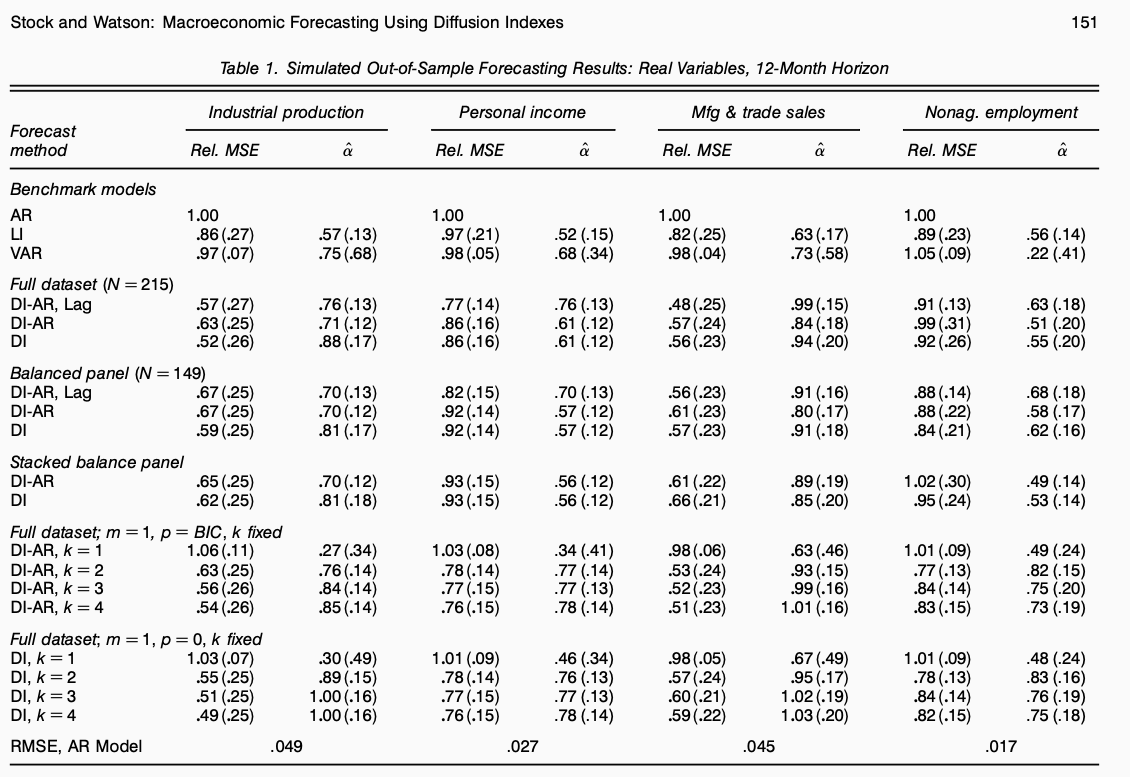
\includegraphics[width=10cm]{pics/stock.png}
        \end{figure}
\end{frame}

\begin{frame}{扩散指数模型的因子估计}
    为了得到因子序列,需要对静态因子进行估计,Stock和Watson采用
    主成分分析作为非参数估计。
    \begin{figure}[H]
        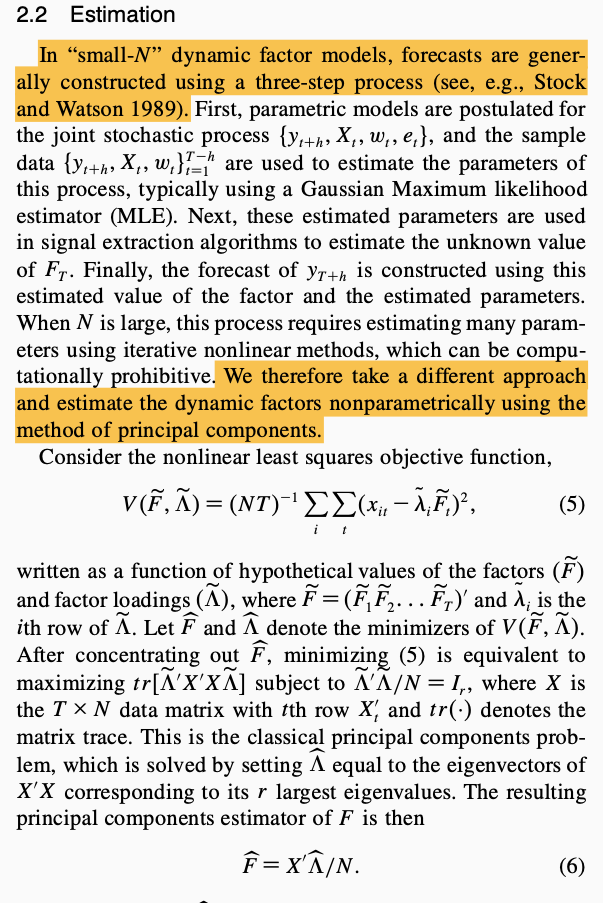
\includegraphics[width=6cm]{pics/stock-principle.png}
        \end{figure}
\end{frame}

\begin{frame}{主成分分析法}
    \begin{itemize}
        \item
        主成分分析法是常见的降维方法。
    \end{itemize}
\end{frame}